\documentclass[11pt]{report}
%\documentclass{foils}

\usepackage{koweydoc}
\usepackage{graphicx}
\usepackage{qtree}

%\usepackage{koweyslide}
\newcommand{\commandline}{\texttt}
\newcommand{\commandgui}{\textit}
\newcommand{\jargon}{\textbf}

\begin{document}
\title{Geni Manual}
\author{Eric Kow\\LORIA}

\maketitle
\tableofcontents

\chapter{Overview}

GenI is a surface realiser for natural language using 

\begin{itemize}
\item the Tree Adjoining Grammar (TAG) formalism 
\item a flat semantic representation
\item a head-driven generation algorithm
\end{itemize}

It runs on Linux and Mac OS X.  It might also run on Windows 
with a little work, but we have not tried.  

In this chapter, we give you a small overview of the generator and an
introductory walkthrough, so that you can get an idea of what the
surface realiser does.  The rest of the manual provides much less
handholding, but more detailed information about using and configuring
the realiser.  

\section{Features}

GenI features 

\begin{enumerate}
\item an optional graphical user interface 
\item a debugger (graphical only)
\item a batch-processing and test suite system
\item a converter from (a variant of) the TAGML format
\end{enumerate}

FIXME: section numbers

\section{Walkthrough}
\label{sec:walkthrough}

\subsection{Getting started}

You can run geni on the command line by executing the command 
\commandline{./geni} from your favourite terminal application.
What appears is the graphical interface\footnote{There is also
a non-interactive text version of the interface, see section 
\ref{sec:configuration_files}}:

% this is how you would include an image in your document
\begin{figure}[h]
\begin{center}
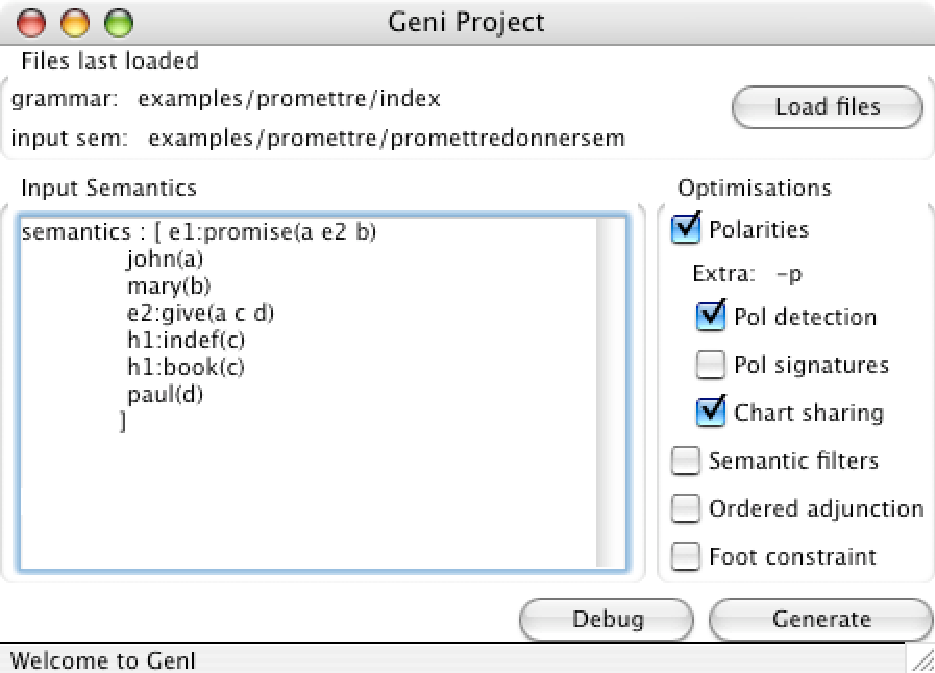
\includegraphics[scale=0.5]{images/geni_gui.pdf}
\label{fig:geni_screenshot}
\end{center}
\end{figure}

The surface realiser takes two inputs: a grammar and a semantic
expression. GenI provides a default grammar and semantics, so
let's take a look at what these inputs produce: click on the 
\commandgui{Generate} button.

What appears, maybe after some seconds of thinking is a results window.
To the see the output, click on the \commandgui{Realisations} tab:  

% this is how you would include an image in your document
\begin{figure}[h]
\begin{center}
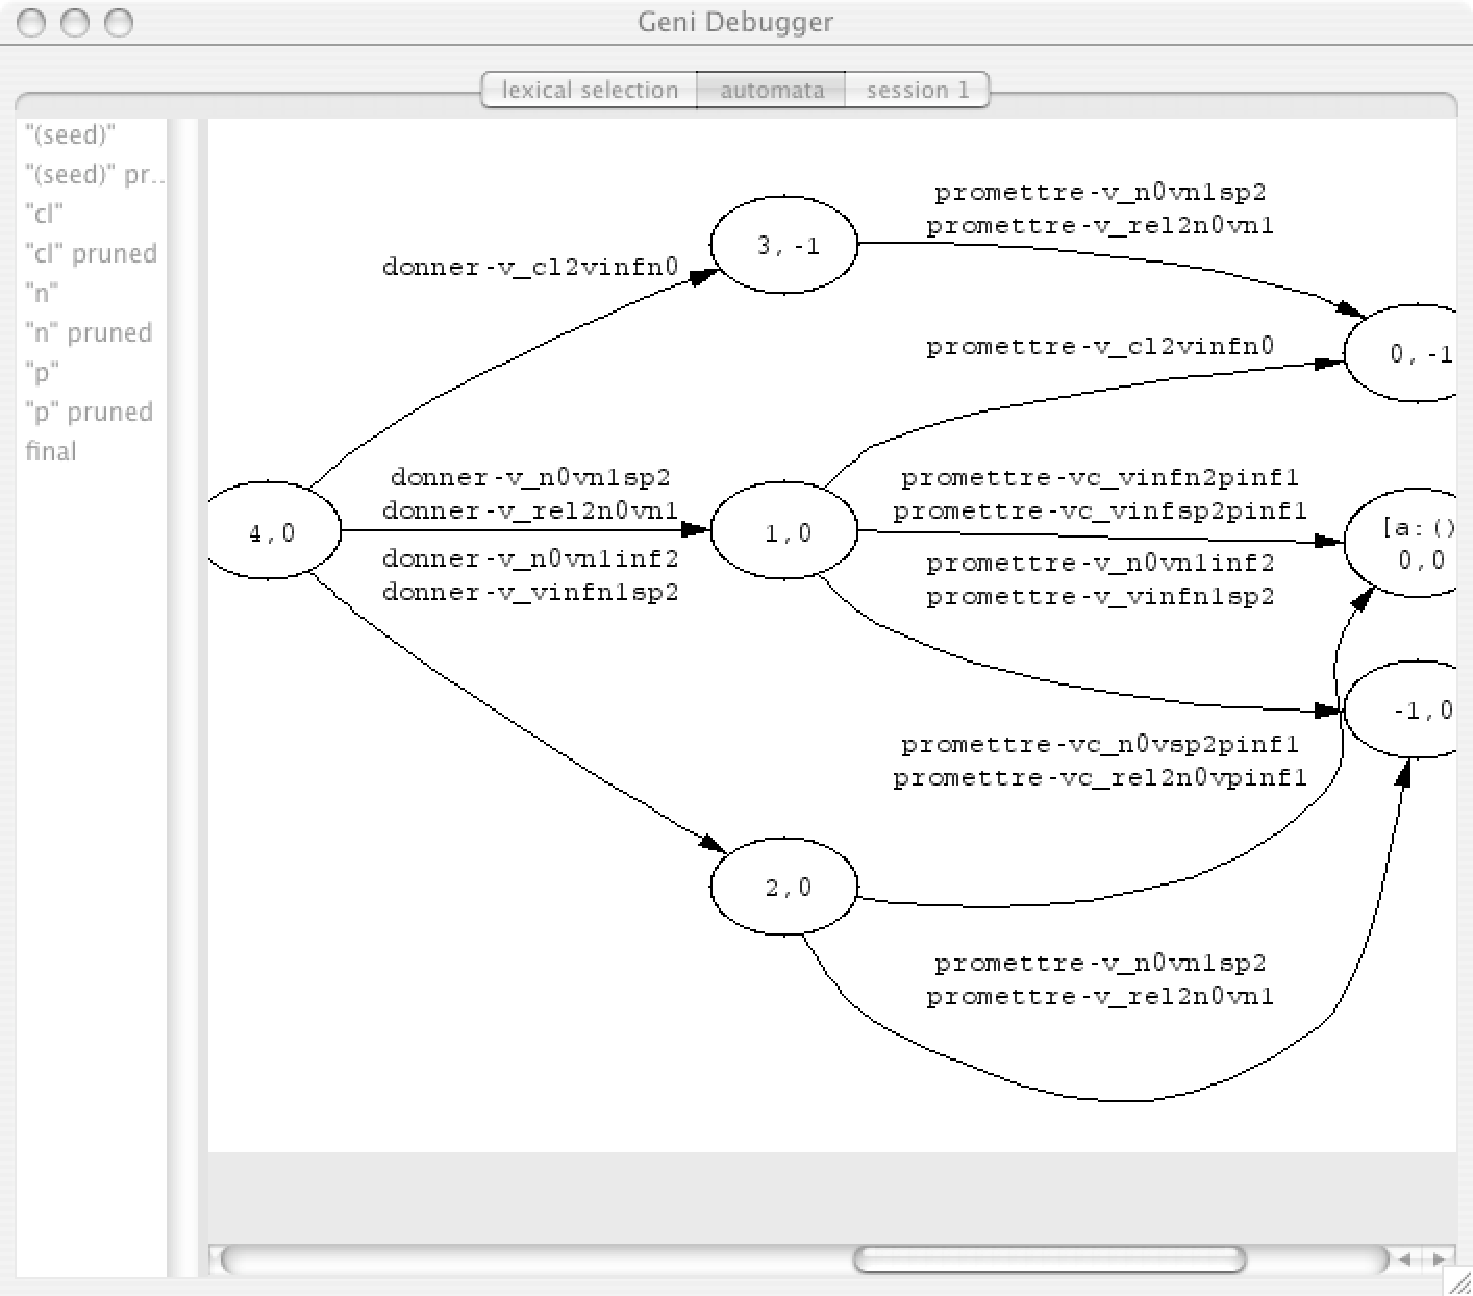
\includegraphics[scale=0.5]{images/geni_polaut.pdf}
\label{fig:geni_results}
\caption{Results: Realisations tab}
\end{center}
\end{figure}

You should see a small number of sentences on the left. If you click on
one of these sentences, its derivation and derived tree will appear on
the right.

Summary so far:

\begin{enumerate}
\item \commandline{./geni}
\item click on \commandgui{Generate}
\item results window: click on \commandgui{Realisations}
\end{enumerate}

Voila! This shows you roughly the kind of things GenI is capable of
doing.  Now in the rest of the walkthrough, we'll see how the realiser
responds to a different input semantics and grammar.

\subsection{Playing with input semantics}

FIXME: to be completed

%\subsection{Input semantics}
%
%You write the input semantics without any commas:
%\begin{verbatim}
%\end{verbatim}
%
%You can also specify handles in the semantics:
%\begin{verbatim}
%\end{verbatim}
%
%Or write recursively embedded semantics:
%\begin{verbatim}
%\end{verbatim}
%
%But if you add handles, please be sure to add them to every literal,
%or GenI could behave unpredicatably.

% ====================================================================
\chapter{Using GenI}
% ====================================================================

FIXME: config file all in one place, but still can tell user bits and
pieces, like set Foo=Bar in .genirc

% ====================================================================
\chapter{Input files}
% ====================================================================

\section{Configuration files}
\label{sec:configuration_files}

GenI configuration consists of a list of
attributes and values of the form Attribute = Value.  For example: 

\begin{verbatim}
Grammars   = foo/index 
TSemantics = foo/chatnoirsem
\end{verbatim}

The basic configuration attributes are

\begin{description}
\item[Grammar]         index files of the Geni grammar
\item[TSemantics, TestSuite] file containing an input semantics or a
                             test suite (mutually exclusive)
\item[Optimisations]   a comma delimited list of optimisations (see
                       section \ref{sec:optimisations}).
\item[ExtraPolarities] a list of default polarities for paraphrase selection   
\end{description}

\subsection{Optimisations}

For a more thorough description of these optimisations, see
\cite{kow2003}.

\subsubsection{Polarity automata}

The first set of optimisations is to filter the lexical selection,
so that only (potentially) syntactically compatible combinations
of trees are given to the generator.  

\begin{description}
\item[PolOpts]   equivalent to Polarised, AutoPol, ChartSharing
\item[Polarised] construct polarity automata at all
\item[AutoPol]   automatically detects polarities from node categories.
                 Warning! You have to use ExtraPolarities for this to
                 work since all trees have a (+) polarity on their 
                 root category.
\item[PolSig]    group trees into polarity signatures, i.e. by their
                 semantics and polarities
\item[PolSort]   when constructing the automaton, first sort the
                 literals of the target semantics by the number
                 of trees which correspond to that literal
\item[ChartSharing] instead of performing a seperate realisation
                    for each automaton path, annotate the trees
                    with their path information and only compare
                    trees on an intersecting set of paths
\end{description}

\subsubsection{Adjunction}

The other optimisations deal with the adjunction phase of the
generator.

\begin{description}
\item[PolOpts]     equivalent to SemFiletered, OrderedAdj, FootConstraint
\item[SemFiltered] before passing to the adjunction phase,
                   first filter out the trees which we know
                   will be semantically incomplete.
\item[OrderedAdj] impose an order on which potential
                  adjunction nodes of a tree are explored
\item[FootConstraint] do not allow the foot node of an auxiliary tree to
                      become an adjunction node after it has been 
                      adjoined into a tree
\end{description}

\subsection{Batch processing}
There are three types of batch processing:
\begin{enumerate}
\item Multi-input:
      You can write multiple configurations in .genirc if you separate
      them by a bang (!).  This will run geni in multiple sessions.
      Each session inherits the configuration of the previous session,
      except for the attributes that you overwrite.  Don't forget to
      unset your ExtraPolarities or Optimisations unless you want them
      to be inherited!
\item Optimisations = Batch 
      Will run geni through all the possible combinations of
      optimisations.  Note that if you specify other optimisations
      in addition to Batch, it will restrict itself to the 
      combinations that include the other optimisations.  For
      example, \texttt{Optimisations = Batch, Polarised} will try
      all combinations of optimisations where Polarities enabled.
      This is useful for performance testing
      of the GenI optimisations.
      N.B. you can use Optimisations=Batch together with multi-input
      if you want.
\item TestSuite - runs the generator over a set of input semantics
      specified in a test suite file; and compares the realisations
      with those expected by the test suite
\end{enumerate}

\subsection{Extra polarties}

The ExtraPolarities argument sets some base polarities when constructing
polarity automata.  

\section{Input semantics}

The input semantics can either be specified in a target semantics file
or as part of a test suite.  

\subsection{Target semantics}

We use a flat representation for the input semantics (although not
neccesarily MRS (FIXME: cite copestake)).  This consists of a set of
literals, where each literal is an (optional) handle, a predicate and
some arguments.  

All of this is written in a block \verb$semantics:[]$,
with spaces as delimiters, not commas.  For example, the following
input semantics file could be realised as ``John promises Paul to give
Mary a book''.

\begin{verbatim}
semantics:[h1:john(j) 
           h2:mary(m) 
           h3:paul(p)
           h3:book(b) h3:indef(b)
           e1:give(j b m) 
           e2:promise(j p e1) 
           ]
\end{verbatim}

\subsection{Test suite}

A test suite can contain more than one input semantics.  Each input
semantics can also be associated with a set of expected realisations:

\begin{verbatim}
semantics:[h1:john(j) h2:mary(m) e1:love(j m) e2:claim(j m e1)]
[ john claims to love mary ]
[ john claims that he loves mary ]

semantics:[h1:john(j) h2:mary(m) 
           h3:book(b) h3:indef(b)
           e1:give(j m b)]
[ john gives a book to mary ]
\end{verbatim}

\subsubsection{Running a test suite}

If you run the generator on a test suite, it will output a summary:
FIXME

\section{Grammar files}

Grammars consist of the following:

\begin{enumerate}
\item index file - which tells where the other files
      in the grammar are (relative to the grammar)
\item semantic lexicon file - semantics $\rightarrow$ lemma
\item syntactic lexicon file - lemma $\rightarrow$ families
\item macros file  - unlexicalised trees
\end{enumerate}

\subsubsection{How GenI uses the grammar}

The surface realiser combines the semantic and syntactic lexicons using
lemma and category as the link between the two.  In other words; an item
in semantic lexicon and one in the syntactic lexicon are considered as
referring to the same lexical entry (\jargon{lexentry}) iff they have
the same lemma and category.  

The lexicon is then consulted for lexical selection in conjuction with
the macros file.  The input to the lexical selection process is a
semantics, and the output is a set of lexicalised tree.  The surface
realiser chooses the lexentries whose semantics subsume the input
semantics.  For each lexentry, it performs unification between the input
semantics and the lexentry semantics; then between the lexentry
semantics and its parameters.  The surface realiser then selects the
tree families associated with the lexentry, and lexicalises all of the
trees within by replacing the anchor node with the lemma and performing
unification between the lexentry parameters, the tree parameters and
tree feature structures.  In short, the propogation of semantic indices
is from input semantics $\rightarrow$ lexentry semantics $\rightarrow$
lexentry parameters $\rightarrow$ tree parameters $\rightarrow$ tree
feature structures.  

\subsection{Index file}

The index file tells the generator where to find all the other parts of
the grammar.  Relative pathnames are based on the index file.  If you do
not specify any path information, the generator will look in the same
directory as the index file.

\paragraph{Example}

\begin{verbatim}
Macros          = macros 
Lexicon         = synlex 
SemanticLexicon = semlex
RootCategories  = s
\end{verbatim}

RootCategories allows you to compensate for automatic polarity
detection.  Since every tree is assigned a $+$ polarity for the category
of its root node, there will be an excess $+r$ charge where r is the
root node for sentences.  If you set \texttt{RootCategories = r}, then
the surface realiser cancels this out by assuming a $-r$ polarity to
begin with.

\subsection{Semantic lexicon}

The semantic lexicon associates semantic entries with lemmas.  Each
entry consists of (1) a lemma and category, (2) a list of parameters
and (3) a semantics

\paragraph{Example}
\begin{verbatim}
le cl (I)
semantics:[]

le det (I) 
semantics:[def(I)]

livre n (I)
semantics:[book(I)]

persuader v (E X Y Z) 
semantics:[E:convince(X Y Z)]
\end{verbatim}

\paragraph{Notes}

\begin{enumerate}
\item a semantics may have more than one predicate
\begin{verbatim}
cher adj (E X Y) 
semantics:[E:cost(X Y) E:high(Y)]
\end{verbatim}
\item a lemma may have more than one distinct semantics

\begin{verbatim}
FIXME: insert example here
\end{verbatim}

\item a semantics may be realised by more than one lexical entry (e.g.
      synonynms)

\begin{verbatim}
livre n (I)
semantics:[book(I)]

bouquin n (I)
semantics:[book(I)]
\end{verbatim}

\end{enumerate}

\subsection{Syntactic Lexicon}

The syntactic lexicon associates each lemma with one or more tree
families.  Each entry consists of (1) a lemma and category (2)
a tree family name.

\paragraph{Example}
\begin{verbatim}
le cl clitic 
le det Det
livre n nC
persuader v vArity3
persuader v vArity3controlObj
\end{verbatim}

\subsection{Macros}

The macros file contains a set of unlexicalised trees organised into
families.  More precisely, the basic components of the file are
families, macros, trees and nodes.  Families contain one or more macros.
Each macro describes a tree, and each tree is composed of nodes.

\paragraph{Families} are written

\begin{verbatim}
begin family name-of-family
% macros
end family
\end{verbatim}

\paragraph{Macros} consist of (1) a name (2) a list of parameters (3) ``initial''
or ``auxiliary'' (4) a tree.  

\paragraph{Trees} are recursively defined structure of form
\verb$node{tree*}$.  For example, the structure 
\verb$n1 { n2 n3 { n4 n5 } n6 }$ should produce the following tree:
\Tree [ .n1 n2 [.n3 n4 n5 ] n6 ]

\paragraph{Nodes} consist of (1) a name (2) a type (optional); and (3)
either a lexeme, or top and bottom feature structures. Here are examples
of the five possible kinds of nodes:

\begin{verbatim}
n1 [cat:n idx:I]![cat:n idx:I]            % basic
n3 type:subst [cat:n idx:Y]![cat:n idx:Y] % subst
n4 type:foot  [cat:n idx:Y]![cat:n idx:Y] % foot
n5 type:lex   "de"                        % coanchor 
n2 anchor                                 % anchor
\end{verbatim}

\subsubsection{Example}

\begin{verbatim}
begin family adj
adj_post(I)  auxiliary
n0[cat:n idx:I det:_]![cat:n idx:I det:minus ]
{ 
  n1 type:foot [cat:n idx:I det:minus]![cat:n idx:I det:minus]
  n2[cat:a]![]
  { 
    n3 anchor 
  }
}

adj_pre(I)  auxiliary
n0[cat:n idx:I det:_ qu:_]![cat:n idx:I det:minus ]
{ 
  n1[cat:a]![]
  { 
    n2 anchor 
  }
  n3 type:foot [cat:n idx:I det:minus]![cat:n idx:I det:minus]
}
end family

begin family vArity2
n0vn1(E X Y) initial
n1[cat:p]![]
{
  n2 type:subst [cat:n idx:X det:plus]![cat:n idx:X]
  n3[cat:v idx:E]![]
  {
    n4 anchor
  }
  n5 type:subst [cat:n idx:Y det:plus]![cat:n idx:Y]
} 
end family
\end{verbatim}

\subsubsection{Format}

A more formal specification of the macros file format is as follows 
(whitespace assumed between items) :

\begin{verbatim}
<mfile>   := <family>*
<family>  := "begin family" <name> <macro>* "end family"

<macro>   := <name> "(" <param>* ")" <initaux> <tree> 
<initaux> := "initial" | "auxiliary"
<tree>    := <node>
           | <node> "{" <tree>* "}" 

<node>    := <name> "anchor" 
           | <name> <typelex> <id>
           | <name> <type> <topfs> "!" <botfs> 
<type>    := "" | "type:subst" | "type:foot"
<typelex> := "type:lex"

<topfs>   := <fs>
<botfs>   := <fs>
<fs>      := "[" <avpair>* "]"
<avpair>  := <id> ":" <id>

<id>      := ([a-z]|[A-Z]|_)*
<name>    := [a-z] <id>
<param>   := (_|[A-Z]) <id>
\end{verbatim}


%:
%
%% this is how you would include an image in your document
%\begin{figure}[h]
%\begin{center}
%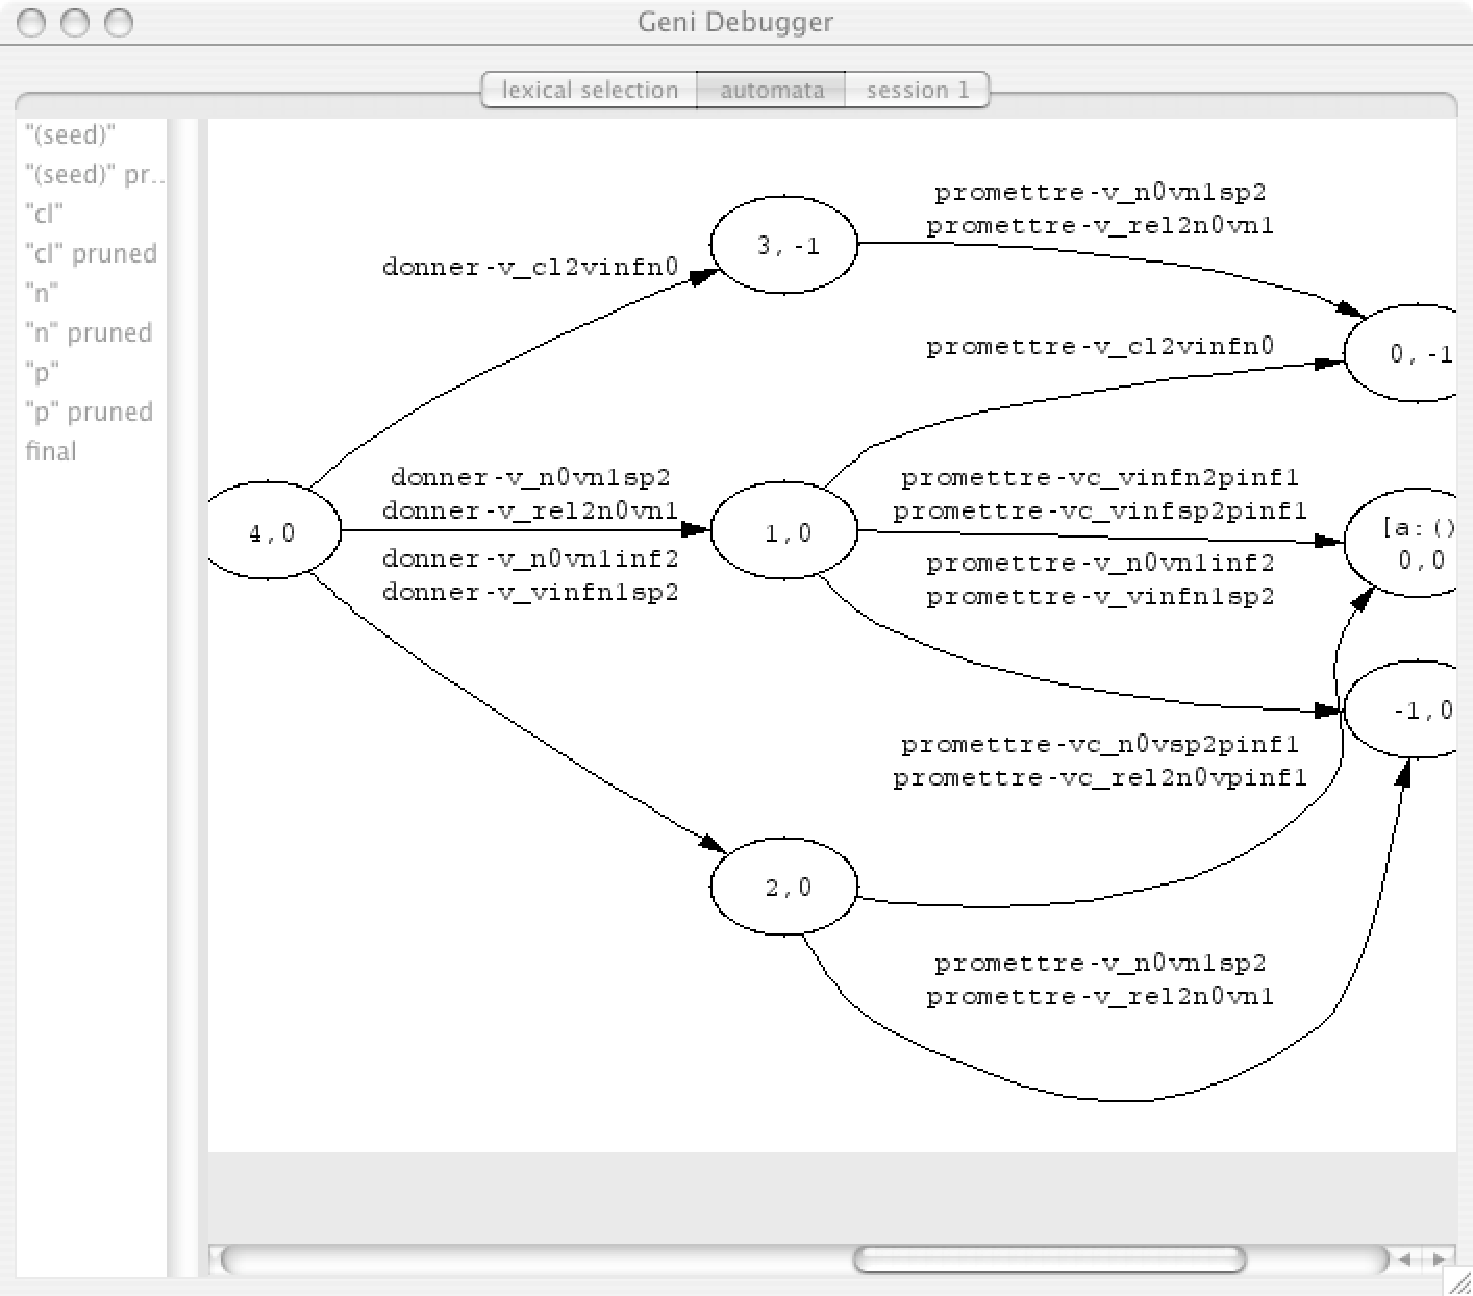
\includegraphics[scale=0.75]{images/geni_polaut.pdf}
%\label{fig:geni_results}
%\caption{Results: Lexical selection}
%\end{center}
%\end{figure}
%
%What you see here is the lexical selection tab.  It shows you the subset
%of the grammar that GenI used for realisation of the input semantics.

%\subsubsection{Polarities}
%
%Polarities mainly go in the macros file.  They appear in the optional
%second parenthesis like so:
%
%\begin{verbatim}
%  IntrV(Event Agent ! agr:A) (+np +np)
%\end{verbatim}
%
%Examples of polarities: +foo, -foo, +3foo, or -3foo

%\subsubsection{TAGML from MGC}
%
%There seems to be no convention for indicating how inflected 
%forms are placed in TAGML tree.  Until somebody tells me 
%otherwise, I am going with the following
%
%\begin{verbatim}
%<node type="none">
%  <fs>
%    <f name="phon">foo</f>
%  </fs>
%</node>
%\end{verbatim}
%
%I refuse to change this until you show me something vaguely
%official-looking.





\end{document}
